% Umschlag AUSFÜHRUNG: helle, serifenbetonte Fassung
\documentclass{standalone}
\usepackage{fontspec}
\usepackage{xcolor}
\usepackage{tikz}

\newfontfamily\serifr{texgyretermes-regular.otf}[
  Path=fonts/,
  BoldFont=texgyretermes-bold.otf,
  ItalicFont=texgyretermes-italic.otf,
  BoldItalicFont=texgyretermes-bolditalic.otf]
\newfontfamily\plexmono{IBMPlexMono-Regular.ttf}[Path=fonts/]
\newfontfamily\plexmonomed{IBMPlexMono-Medium.ttf}[Path=fonts/]

\definecolor{bg}{HTML}{F7F5EF}      % warmes Papier
\definecolor{txt}{HTML}{1B1B1A}     % fast Schwarz
\definecolor{rulecol}{HTML}{D8D5CD} % Haarlinie
\definecolor{promptc}{HTML}{8B887F} % $-Prompt, gedämpft
\definecolor{outc}{HTML}{3A3A38}    % Ausgabe-Zeile, dunkelgrau

\begin{document}
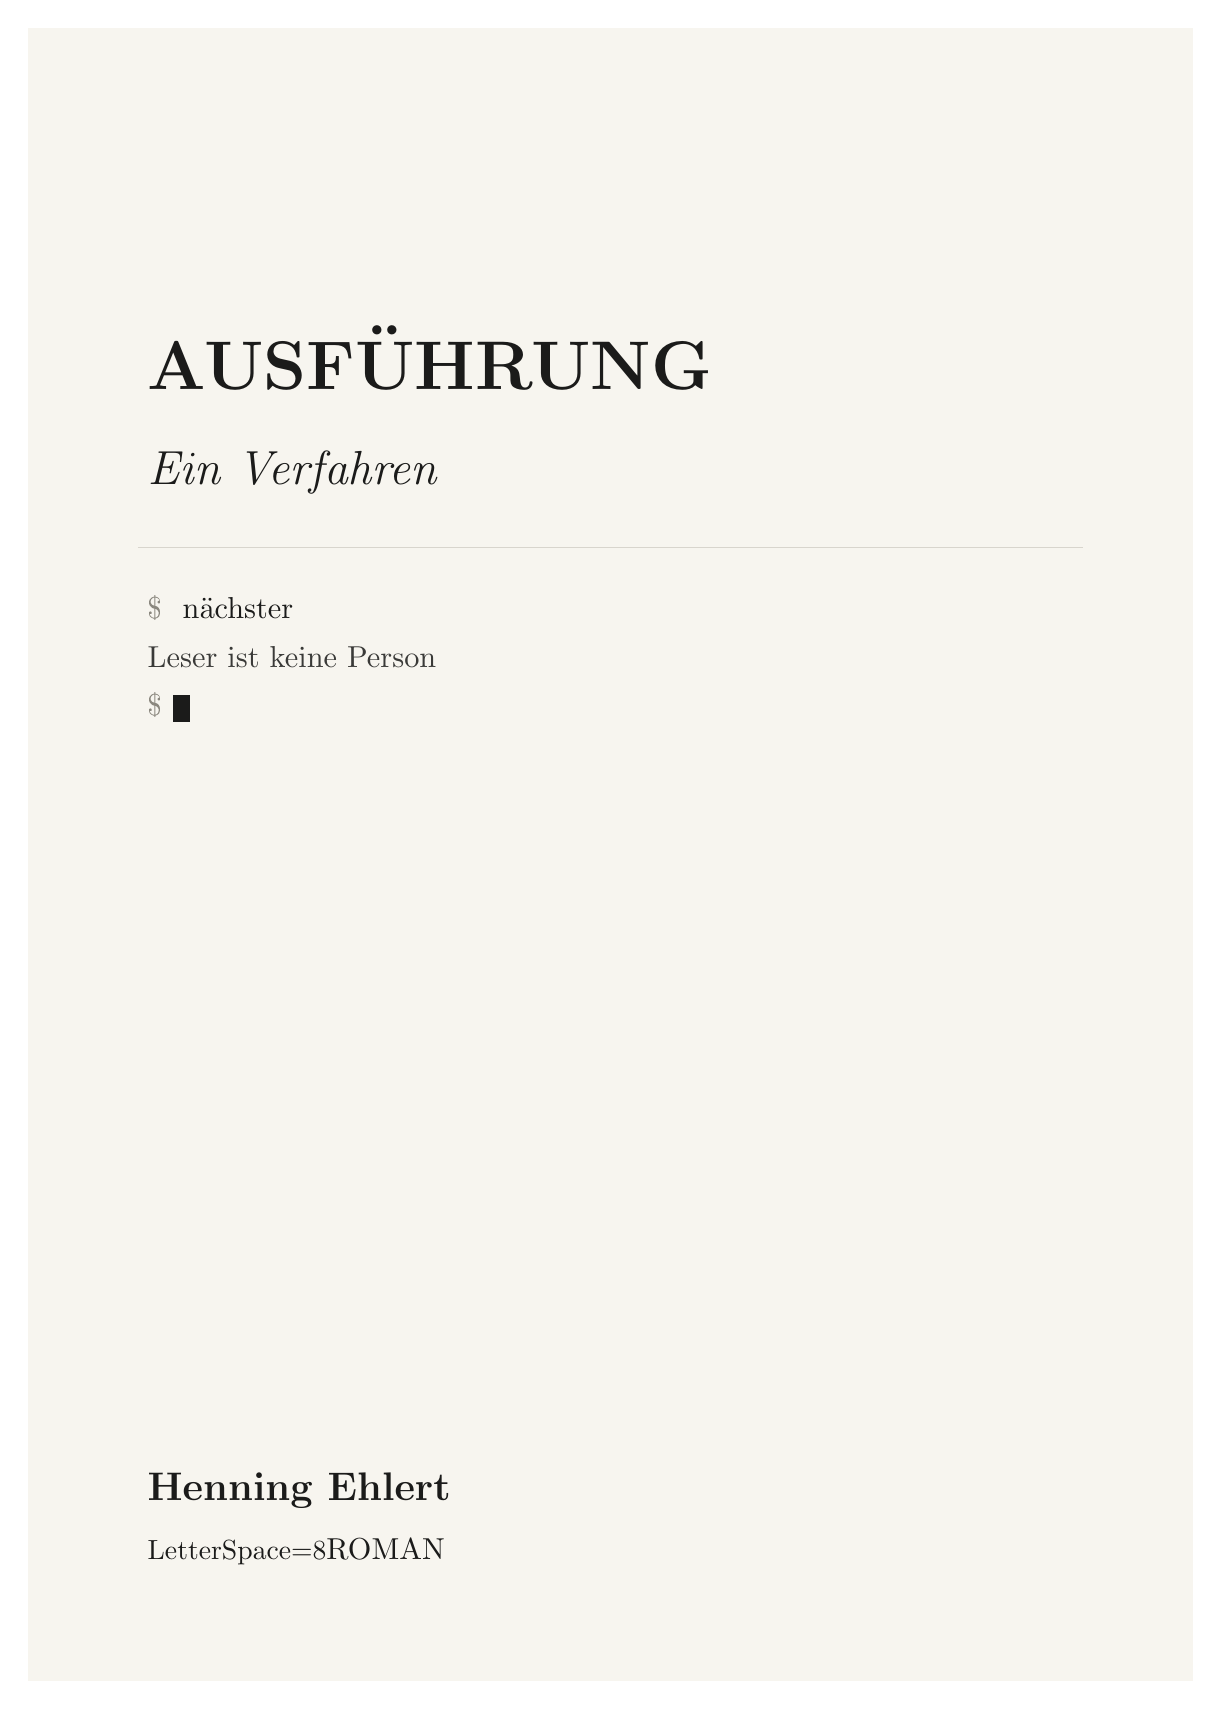
\begin{tikzpicture}[x=1mm,y=1mm]
  \useasboundingbox (0,0) rectangle (148,210);
  \fill[bg] (0,0) rectangle (148,210);

  % Titel
  \node[anchor=base west] at (14,164)
    {\color{txt}\serifr\bfseries\fontsize{49bp}{49bp}\selectfont AUSFÜHRUNG};

  % Untertitel
  \node[anchor=base west] at (14,152)
    {\color{txt}\serifr\itshape\fontsize{16bp}{16bp}\selectfont Ein Verfahren};

  % Haarlinie
  \draw[rulecol, line width=0.4bp] (14,144) -- (134,144);

  % Terminal-Zeilen — ohne Box, direkt auf dem Papier
  \node[anchor=base west] at (14,135)
    {\color{promptc}\plexmono\fontsize{10.5bp}{10.5bp}\selectfont \$};
  \node[anchor=base west] at (18.445,135)
    {\color{txt}\plexmonomed\fontsize{10.5bp}{10.5bp}\selectfont nächster};
  \node[anchor=base west] at (14,128.8)
    {\color{outc}\plexmono\fontsize{10.5bp}{10.5bp}\selectfont Leser ist keine Person};
  \node[anchor=base west] at (14,122.6)
    {\color{promptc}\plexmono\fontsize{10.5bp}{10.5bp}\selectfont \$};
  \fill[txt] (18.445,121.785) rectangle (20.6675,125.304);

  % Autor / Gattung — zwischen Titel- und Mono-Größe, unten auf der Seite
  \node[anchor=base west] at (14,23)
    {\color{txt}\serifr\bfseries\fontsize{14bp}{14bp}\selectfont Henning Ehlert};
  \node[anchor=base west] at (14,15.5)
    {\color{txt}\plexmono\addfontfeature{LetterSpace=8}\fontsize{10.5bp}{10.5bp}\selectfont ROMAN};

\end{tikzpicture}
\end{document}
